\chapter{Platform}
\label{chp:Platform}
A device has been made to generate, receive and analyse flashes. The complete system architecture can be found in figure \ref{fig:systemOveriew}. Each component and their interfaces will be discussed briefly, followed by a section showing the final build of the platform.

\begin{figure}[h]
	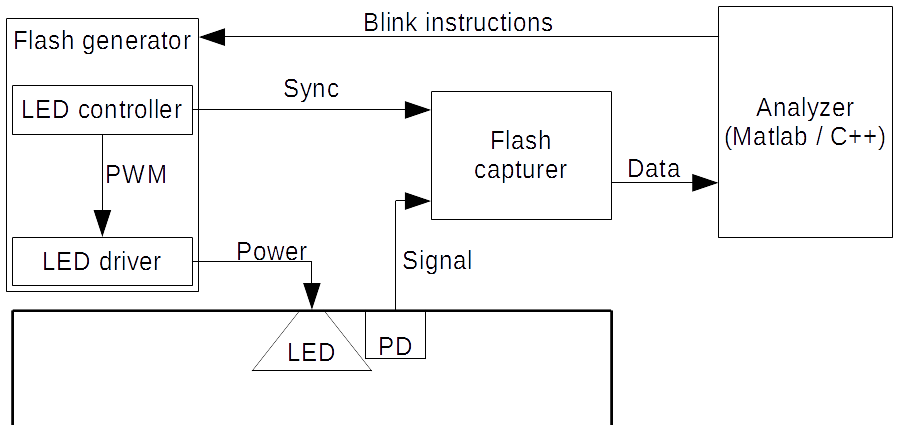
\includegraphics[width=\textwidth]{pics/systemOverview.png}
	\caption{System architecture of the flash generator/analyser}
	\label{fig:systemOveriew}
\end{figure}

\section{system components}

\subsection{Flash generator}
The flash generator is a device able to control a LED with high precision. It is able to set the period $T$, and the t-on time $T_{on}$. $T$ Controls the frequency of the flashes and $t_{on}$ length. Both parameters can be set with a resolution of $10\mu s$ resulting in a precisely controlled PWM signal with the help of equation \ref{eq:1/f=T}. This signal is sent to a LED driver trough one of three LED drivers, which will make the actual light turn on and off at different light levels.

Besides generating the PWM signal for the light, the flash generator has another function. It sends a sync signal to the flash receiver just before generating a flash. This allows the Flash generator to be ready when the flash starts, so it does not waste time sampling if no flash is generated.

\begin{equation}
\label{eq:1/f=T}
T=\frac{1}{f}
\qquad
DutyCycle=\frac{T_{on}}{T} * 100\%
\end{equation}

%\begin{figure}[]
%	\centering
%	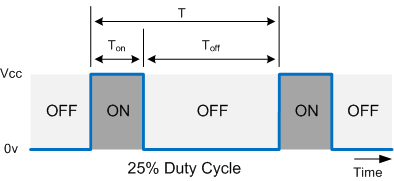
\includegraphics[]{pics/DutyCycle.png}
%	\caption{Visualization of how $T$ and $T_{on}$ determine the duty cycle and frequency of the flash generator}
%	\label{fig:DutyCycle}
%\end{figure}

\subsection{Reflection receiver}
The job of the receiver is to sample values while the light is being turned on and off, to then analyse the full flash and extract it's features. The receiver should capture flashes as precise and consistent as possible. For this reason, the receiver receives a sync signal from the flash generator, so it can start sampling at exactly the same moment every time relative to the start of the flash. 

The receiver should continue sampling until the light has completely turned off. once done, the device should do one of the following things, depending on the mode of the analyser:
\begin{enumerate}[itemsep=-1ex]
	\item Send back the full flash, uncompressed, for analysis of separate flashes.
	\item Send back all compressed flashes, by extracting several features.
\end{enumerate}

\subsection{Analyser}
The analyser will receive samples from the reflection receiver and is ran on a PC in the form of either a C/C++ program (real-time) or as a MATLAB script (post-time). The analyser can set the receiver to raw-. or compressed mode. If the receiver sends raw flashes to the analyser it can be used to analyse this flash. This mode is used in chapter \ref{sec:Flash_characteristics} to analyse single flashes to find the ideal settings for the flash generator and reflection receiver. If the receiver sends compressed flashes, the analyser is able to analyse consecutive flashes. This mode will be used in chapter \ref{sec:Algorithm} to find an algorithm to determine if an object is moving in the area under the light.

The Analyser should also be able to control the flash generator if the system is running in real-time mode. It is therefore able to send a packet with $T$, ${T_on}$ and $I_{LED}$ to the device. This allows for real time control of the flash generator.

\section{Implementation}
The system was build by combining several of shelve parts. An overview of the actual build can be seen in figure \ref{fig:acutalBuild}. It shows the different components mounted on a box. This section will explain briefly how each system component is implemented and why each part was chosen.

The flash generator is implemented on an Arduino UNO\cite{ArduinoUno}. This platform was chosen, as it's simple to use, does not require an operating system (OS) and has therefore no unexpected jitter. The LED used in the set-up is the same LED as modelled in chapter\ref{Model}\cite{lamptest}. The power settings of the LED's where chosen after some experimentation with the flash generation and reception and can be seen in equation \ref{eq:Power}.

\begin{equation}
\label{eq:Power}
P_{LED}=\frac{(V_{DD} - U_{LED})^2}{R}
\qquad
P_{LED} = \frac{(7.2 - 3.6)^2}{[1, 3, 5]} = [4W, ,1.33W]
\end{equation}

The reflection receiver is implemented on the shine platform \cite{Shine}. This platform was chosen because it's a simple (no OS required) hands-on platform featuring multiple photo diodes by default. A downside of the shine platform is that it's unable to communicate directly with a computer as it does not has a FTDI interface. This problem was solved by using a processor-less Arduino UNO as bridge between the analyser and shine platform.

The receiver makes use of three photo diodes. The original sensors on shine where replaced with ones more sensitive to visible light. Each sensor is also configured in a different way. Some feature an increased amplification of the measured signal. Others have a longer wire with (intentional) bad shielding to simulate how the system does in a environment with a lot of electromagnetic radiation. An overview of the PD configurations can be seen in table \ref{tbl:PDs}.

\begin{table}[]
	\centering
	\label{tbl:PDs}
	\begin{tabular}{clll}
		PD\#                   & Wire lenght & Sensitivity & EMC Shield \\ \cline{2-4} 
		\multicolumn{1}{c|}{1} & Long        & Normal      & Slecteable \\
		\multicolumn{1}{c|}{2} & Short       & Normal      & Yes        \\
		\multicolumn{1}{c|}{3} & Short       & Normal*1000 & Yes       
	\end{tabular}
	\caption{Overview of photo diode configurations}
\end{table}

\begin{figure}
	\centering     %%% not \center
	\subfigure[Top view]{\label{fig:top}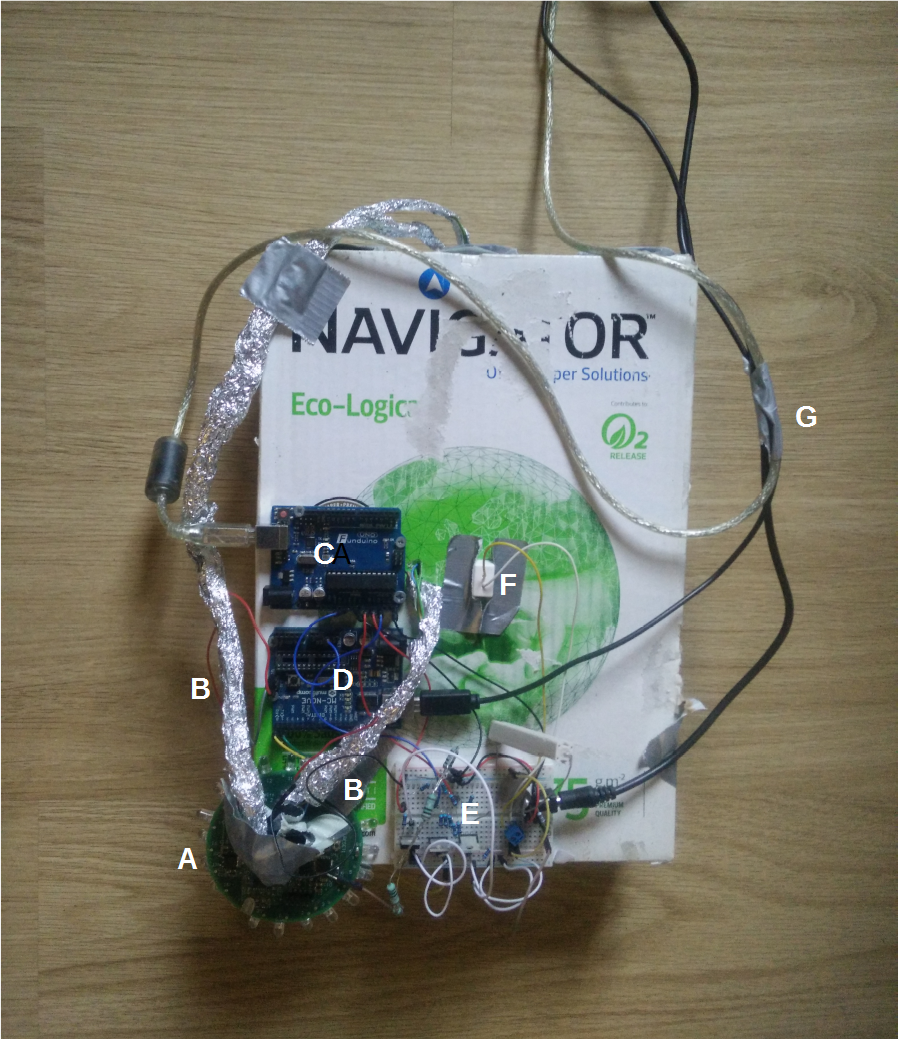
\includegraphics[width=60mm]{pics/platform_top.png}}
	\subfigure[Bottom view]{\label{fig:bot}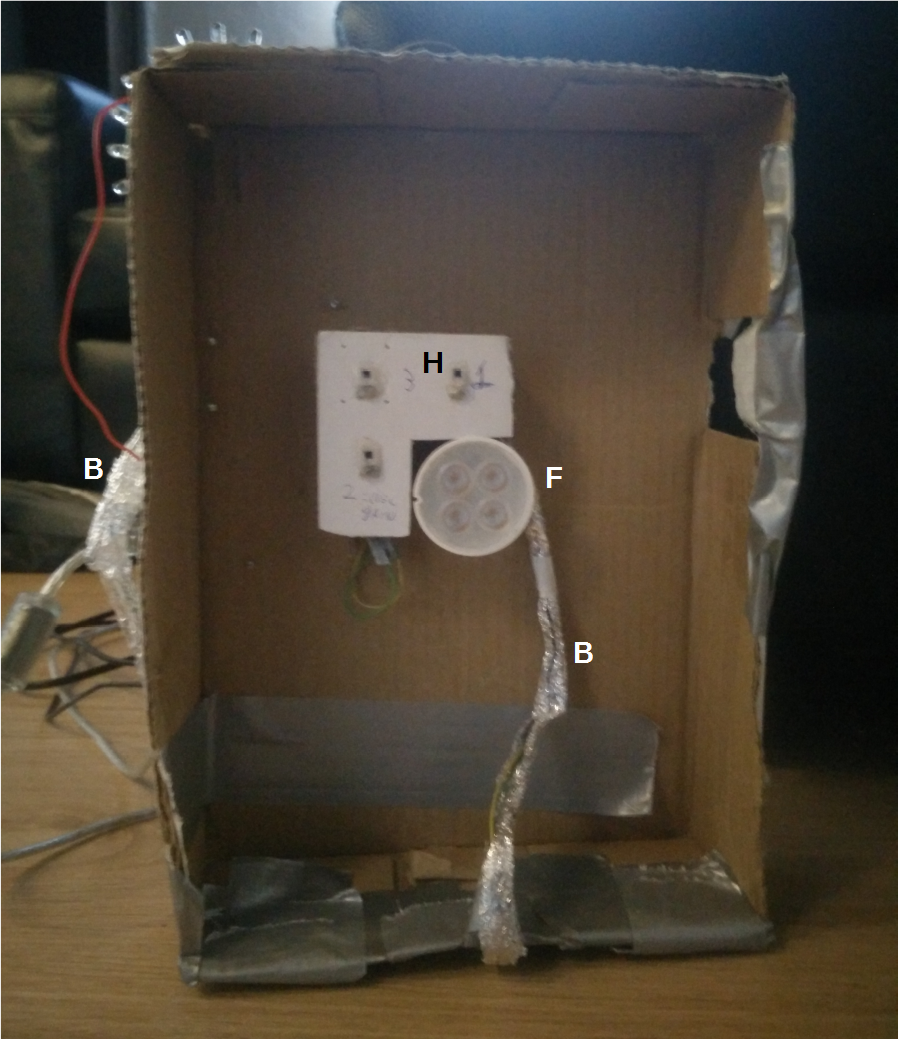
\includegraphics[width=60mm]{pics/platform_bot.png}}
	\captionsetup{singlelinecheck=off}
	\caption[]{The platform prototype. Each letter denotes a different component:
		\begin{enumerate}[label=\Alph*,itemsep=-1ex,topsep=0pt]
			\item = Reflection receiver
			\item = Wires to the photo diodes
			\item = LED controller
			\item = Communication bridge between shine and the PC
			\item = LED driver
			\item = The LED
			\item = Wires to the analyser and power supply
			\item = Three photo diodes
	    \end{enumerate}}
    	\label{fig:acutalBuild}
\end{figure}

\section{Evaluation}
The system has been build and tested. Several captured test flashes can be seen in figure \ref{fig:FristFlashes}. Even though the created device has a poor build quality, it has great potential for experimentation with the proposed method of activity detection. The main advantages are:
\begin{itemize}[itemsep=-1ex]
	\item Each building block has one clear purpose and can therefore be tackled separately from other components. It's therefore impossible that a timing error in the flash generator software affects the sampling of the receiver or vice versa.
	\item The build quality is poor. If the project works on this device, it will definitely work on a dedicated platform.
\end{itemize}
The next steps for the project is finding a method for extracting useful information from flashes as shown in figure \ref{fig:FristFlashes}. 

\begin{figure}
	\centering     %%% not \center
	\label{fig:FristFlashes}
    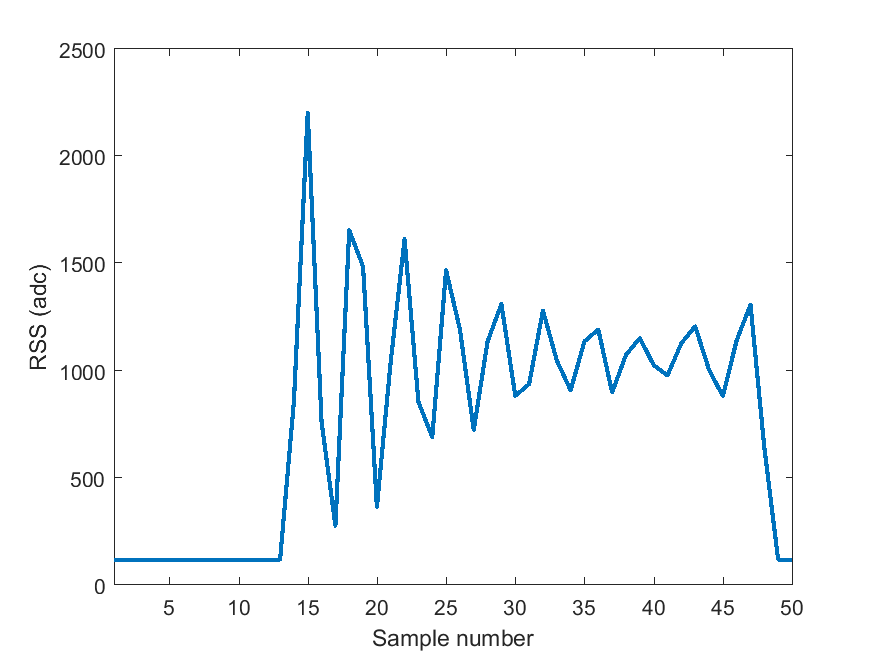
\includegraphics[width=90mm]{pics/no_filter.png}
	\caption{One of the first received  with the experimental platform.}
\end{figure}